
\section{Evaluation}\label{sec:evaluation}

Before we discuss evaluation, we should have some goals set up. This is necessary because evaluation results can be compared against the goals in order to
conclude whether all goals are met or not. As stated in section~\ref{section:aims}, our goal is to integrate new kind of expertise evidence, funded projects,
with existing expertise evidence, publications to enhance the performance of the retrieval system. At the end of this section, we have to be able to 
answer the following questions:

\begin{itemize}
 \item Does integrating funded projects with publications using learning to rank technique (LETOR) help improve the performance of the retrieval system?
\end{itemize}


\subsection{Experimental Setting}
This section is aimed to demonstrate that applying LETOR techinque improves the performance of the retrieval system. To evaluate this, we use LETOR
technique proposed in section~\ref{sec:letor}. Basically, there are 2 datasets: training and testing datasets. In IR, 
we refer them as training and testing queries. The following is a list of steps in running an evaluation:
\begin{enumerate}
 \item generate a LETOR file for testing queries.
 \item from the LETOR file obtained from (1), generate a qrels file as discussed in section~\ref{sec:treceval}.
 \item generate 2 learned models~\ref{section:producelearnedmodel} from training queries using AdaRank, and Coordinate Ascent algorithms.
 \item apply each learned model to all testing queries.
 \item for each test in (4), generate a score file of each test using RankLib~\ref{section:rankLib} and generate a result file in TREC format~\ref{sec:treceval}
 \item evaluate each test using trec\_eval~\ref{sec:treceval}
\end{enumerate}

To evaluate without using LETOR (using only publications as expertise evidence), we can set other features apart from publication query feature to 0
and perform step (5) and (6).

%After a learned model has been generated using training queries~\ref{section:producelearnedmodel},
\subsubsection{Training Queries}
34 queries shown in table ~\ref{table:trainingqueries} are used for training. They are trained by the tool called RankLib (section~\ref{section:rankLib}) to get a learned model. 
This process is performed only one time.
\begin{table}
\centering
\begin{tabular}{|c|l|c|l|}
\hline \textbf{\#} & \textbf{Query} & \textbf{\#} & \textbf{Query} \\
\hline 1 & language modelling & 18 & game theory\\
\hline 2 & manets & 19 & stable marriage \\
\hline 3  & match & 20 & quantum computation\\ 
\hline 4  & multimodal & 21 & constraint modelling\\ 
\hline 5  & music as navigation cues & 22 & home networks\\ 
\hline 6  & networking security & 23 & wireless sensor networks\\ 
\hline 7  & neural network & 24 & distributed systems\\ 
\hline 8  & older adults use of computers & 25 & operating system\\ 
\hline 9  & parallel logic programming & 26 & terrier\\ 
\hline 10  & query expansion & 27 & text searching\\ 
\hline 11  & road traffic accident statistics & 28 & trec collection class\\ 
\hline 12  & shoogle & 29 & usability\\ 
\hline 13  & skill-based behavior & 30 & utf support terrier\\ 
\hline 14  & sound in multimedia human-computer interfaces & 31 & visual impairment\\ 
\hline 15  & statistical inference & 32 & wafer fab cost \\ 
\hline 16  & suffix tree & 33 & database\\ 
\hline 17  & mobile hci & 34 & programming languages\\ 
\hline
\end{tabular}
\caption{Training Queries} \label{table:trainingqueries}
\end{table}

\subsubsection{Testing Queries}
33 queries are used for testing as shown in table~\ref{table:testingqueries}.
\begin{table}
\centering
\begin{tabular}{|c|l|c|l|}
\hline \textbf{\#} & \textbf{Query} & \textbf{\#} & \textbf{Query} \\
\hline 1 & empirical methods & 18 & 3d human body segmentation\\
\hline 2 & eurosys 2008 & 19 & anchor text \\
\hline 3  & facial reconstruction & 20 & clustering algorithms\\ 
\hline 4  & force feedback & 21 & different matching coefficients\\ 
\hline 5  & functional programming & 22 & discrete event simulation\\ 
\hline 6  & glasgow haskell compiler & 23 & discrete mathematics\\ 
\hline 7  & grid computing & 24 & distributed predator prey\\ 
\hline 8  & artificial intelligence & 25 & divergence from randomness\\ 
\hline 9  & computer graphics & 26 & ecir 2008 \\
\hline 10  & robotics & 27 & group response systems\\ 
\hline 11  & data mining & 28 & handwriting pin\\ 
\hline 12  & computer vision & 29 & haptics\\ 
\hline 13  & information security & 30 & haptic visualisation\\ 
\hline 14  & 3d audio & 31 & hci issues in mobile devices\\ 
\hline 15  & expert search & 32 & human error health care \\ 
\hline 16  & information retrieval & 33 & information extraction\\ 
\hline 17  & machine translation &  & \\ 
\hline
\end{tabular}
\caption{Testing Queries} \label{table:testingqueries}
\end{table}

\subsection{Experimental Results}

\begin{table}
\centering
\begin{tabular}{|c|c|c|c|c|}
\hline \textbf{Algorithm} & \textbf{MAP} & \textbf{NDCG} & \textbf{MRR} & \textbf{Number of Relevant Experts}\\
\hline AdaRank & 0.0153 & 0.1872 & 0.0116 & 106\\
\hline Coordinate Ascent & 0.5264 & 0.6618 & 0.6332 & 106 \\
\hline Without LETOR  & 0.5499 & 0.6871 & 0.6484 & 106\\ 
\hline
\end{tabular}
\caption{Evaluation Results} \label{table:evaluationresult}
\end{table}

Table~\ref{table:evaluationresult} shows the retrieval performance of the proposed LETOR techniques and without LETOR techinque. It can be clearly seen
that without LETOR gives the performance among other approaches considering MAP, NDCG and MRR evaluating metrices. Coordinate Ascent gives second best 
performance. Therefore, the answer to question is NO, using LETOR technique does not enhance ther performance of the retrieval system.

\begin{table}
\centering
\begin{tabular}{|l|c|c|c|c|c|c|}
\hline \textbf{Testing Queries} & \multicolumn{2}{|c|}{\textbf{AdaRank}} & \multicolumn{2}{|c|}{\textbf{Coordinate Ascent}} & \multicolumn{2}{|c|}{\textbf{Without LETOR}} \\
\hline 				 & \textbf{MAP} & \textbf{MRR}  & \textbf{MAP} & \textbf{MRR}  & \textbf{MAP} & \textbf{MRR} \\
\hline 3d audio & 0.0053 & 0.0053 & 1.0000 & 1.0000 & 1.0000 & 1.0000 \\
\hline 3d human body segmentation & 0.0127 & 0.0068 & 0.1452 & 0.2000 & 0.1824 & 0.2000 \\
\hline anchor text & 0.0263 & 0.0088 & 0.7894 & 1.0000 & 0.7894 & 1.0000 \\
\hline artificial intelligence & 0.0344 & 0.0233 & 0.5944 & 1.0000 & 0.5972 & 1.0000 \\
\hline clustering algorithms & 0.0166 & 0.0071 & 0.3048 & 0.2000 & 0.3048 & 0.2000 \\
\hline computer graphics & 0.0047 & 0.0047 & 0.5000 & 0.5000 & 0.5000 & 0.5000 \\
\hline computer vision & 0.0142 & 0.0130 & 0.4611 & 0.5000 & 0.4611 & 0.5000 \\
\hline data mining & 0.0181 & 0.0118 & 0.9167 & 1.0000 & 0.9167 & 1.0000 \\
\hline different matching coefficients & 0.0091 & 0.0063 & 0.5833 & 0.5000 & 0.5833 & 0.5000 \\
\hline discrete event simulation & 0.0078 & 0.0078 & 0.3333 & 0.3333 & 0.3333 & 0.3333 \\
\hline discrete mathematics & 0.0164 & 0.0115 & 0.0306 & 0.0400 & 0.1394 & 0.1250 \\
\hline distributed predator prey & 0.0058 & 0.0058 & 0.0037 & 0.0037 & 0.1111 & 0.1111 \\
\hline divergence from randomness & 0.0124 & 0.0058 & 0.9167 & 1.0000 & 0.9167 & 1.0000 \\
\hline ecir 2008 & 0.0152 & 0.0070 & 0.8125 & 1.0000 & 0.8125 & 1.0000 \\
\hline empirical methods & 0.0189 & 0.0072 & 0.2092 & 0.1667 & 0.2154 & 0.1667 \\
\hline eurosys 2008 & 0.0055 & 0.0055 & 1.0000 & 1.0000 & 1.0000 & 1.0000 \\
\hline expert search & 0.0107 & 0.0075 & 0.5037 & 1.0000 & 0.5227 & 1.0000 \\
\hline facial reconstruction & 0.0039 & 0.0039 & 0.0021 & 0.0021 & 0.2000 & 0.2000 \\
\hline force feedback & 0.0073 & 0.0050 & 0.6429 & 1.0000 & 0.6250 & 1.0000 \\
\hline functional programming & 0.0244 & 0.0112 & 0.1687 & 0.2000 & 0.2038 & 0.1429 \\
\hline glasgow haskell compiler & 0.0101 & 0.0101 & 0.3333 & 0.3333 & 0.5000 & 0.5000 \\
\hline grid computing & 0.0123 & 0.0083 & 0.3095 & 0.3333 & 0.3333 & 0.3333 \\
\hline group response systems & 0.0054 & 0.0054 & 0.5000 & 0.5000 & 0.5000 & 0.5000 \\
\hline handwriting pin & 0.0054 & 0.0038 & 1.0000 & 1.0000 & 1.0000 & 1.0000 \\
\hline haptic visualisation & 0.0224 & 0.0102 & 0.6111 & 1.0000 & 0.5861 & 1.0000 \\
\hline haptics & 0.0407 & 0.0133 & 0.4929 & 0.5000 & 0.5819 & 0.5000 \\
\hline hci issues in mobile devices & 0.0268 & 0.0091 & 0.5821 & 1.0000 & 0.6160 & 1.0000 \\
\hline human error health care & 0.0064 & 0.0064 & 0.5821 & 1.0000 & 0.3333 & 0.3333 \\
\hline information extraction & 0.0069 & 0.0050 & 0.3333 & 0.3333 & 0.2500 & 0.2500 \\
\hline information retrieval & 0.0308 & 0.0102 & 0.7496 & 1.0000 & 0.7468 & 1.0000 \\
\hline information security & 0.0163 & 0.0120 & 0.7333 & 1.0000 & 0.7333 & 1.0000 \\
\hline machine translation & 0.0117 & 0.0118 & 1.0000 & 1.0000 & 1.0000 & 1.0000 \\
\hline robotics & 0.0404 & 0.1111 & 0.5565 & 1.0000 & 0.5523 & 1.0000\\
\hline

\end{tabular}
\caption{Evaluation Results of Each Testing Query} \label{table:eachqueryevaluationresult}
\end{table}

Table~\ref{table:eachqueryevaluationresult} shows the evaluation results of each testing query. It has shown that similar to Table~\ref{table:evaluationresult},
without LETOR technique is better than using LETOR technique.

\subsection{User Interface of New System}

\begin{figure}
 \centering
 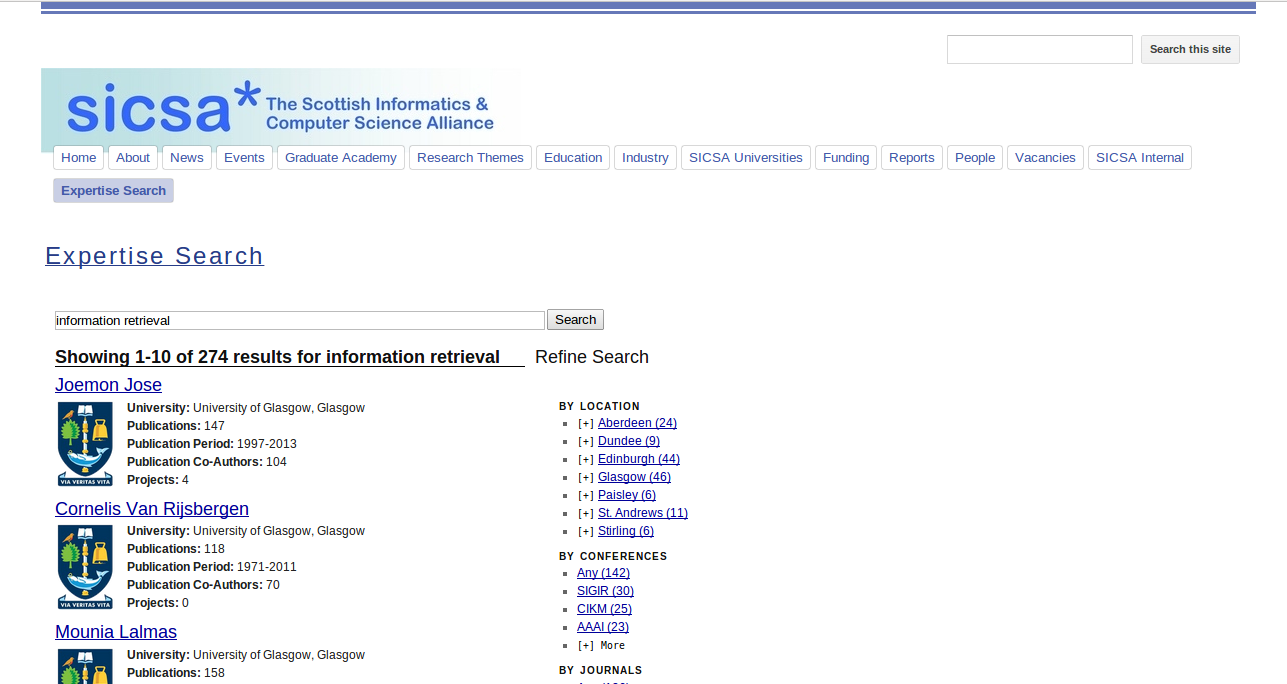
\includegraphics[width=13cm,height=15cm,keepaspectratio]{./figures/newsearch.png}
 \caption{New Facets : Experts In Response to ``information retrieval'' Query} \label{fig:newsearch} 
 \end{figure}
 Figure~\ref{fig:newsearch} shows a new facet in response to a query ``information retrieval''. The number of 
projects experts have been involved in is displayed. In addition to the current system filter modes, filter options by using projects, publications and both
expertise evidence, and by projects' total funding are added on the right panel of the page.

 \begin{figure}
 \centering
 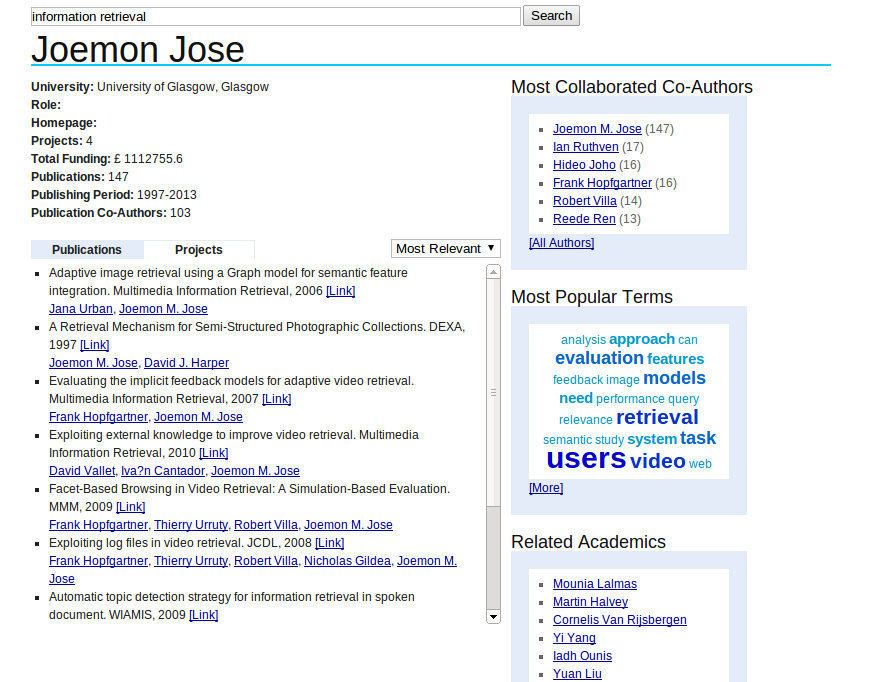
\includegraphics[width=13cm,height=15cm,keepaspectratio]{./figures/newProfilePagePublication.png}
 \caption{New Expert's Profile Facet} \label{fig:newProfilePage} 
 \end{figure}
 Figure~\ref{fig:newProfilePage} shows a new facet of profile page. There are 2 tabs for publications and funded projects and a drop down box for selecting
 result filter modes. The number of projects, project collaborators, project period and total funding are shown.
 
 \begin{figure}
 \centering
 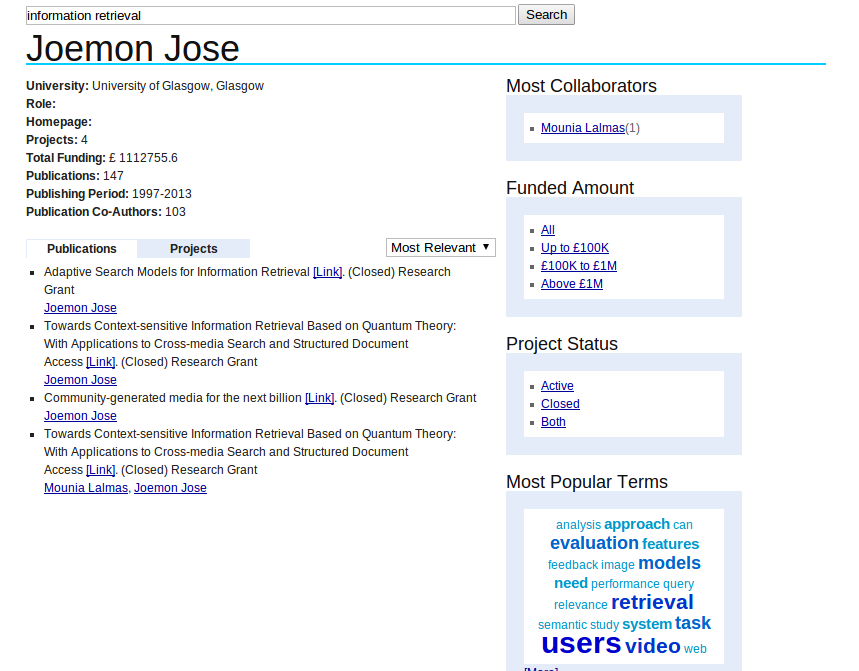
\includegraphics[width=13cm,height=15cm,keepaspectratio]{./figures/newPofilePageProject.png}
 \caption{Project Tab} \label{fig:newPofilePageProject} 
 \end{figure}
 Figure~\ref{fig:newPofilePageProject} shows a facet when a project tab is selected. The right hand side of the page shows the most project collaborators
 and other filter modes: filter projects by amount of funding and by the status of projects.
 
 \begin{figure}
 \centering
 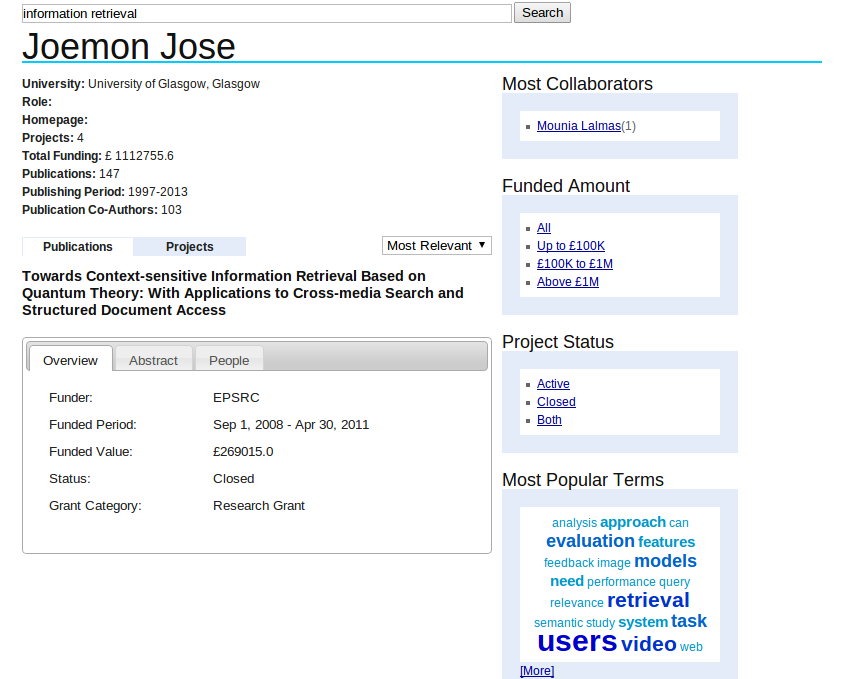
\includegraphics[width=13cm,height=15cm,keepaspectratio]{./figures/newProfileSelectedProject.png}
 \caption{Project Page} \label{fig:newProfileSelectedProject} 
 \end{figure}
 
 Figure~\ref{fig:newProfileSelectedProject} shows a facet when user selects a project link. This shows descriptions of a selected project.
 The descriptions include:
 \begin{itemize}
  \item Funder
  \item Title
  \item Funded Value
  \item Funded Period
  \item Status
  \item Grant Category
  \item People involved in the project
  \item Abstract
  \item Impact
 \end{itemize}
 Some projects descriptions are not shown if they are missing.